\chapter{Specification}
The following section is from our specification made in the beginning of the course.\\
\begin{center}
\textbf{\HUGE Digital distanceinstrument}\\
\end{center}
\subsection{Idea}
The scope of the project is to develop and implement an instrument using distance sensors to a DSP playing different amplitudes and/or frequencies depending on the distance to a hand.\\
\subsection{Scope/preliminary:}
SKAL EVT FLYTTES??
We want to implement our own distance sensor and play different frequencies depending on the distance to an object. We want to use and learn about the analog devices blackfin DSP since we have not encountered it before. We want to use sound as a method of measuring distance. We have never worked with sound outputs and inputs before.\\
\subsection{System overview:}
Below is shown a sketch of the system using simple blocks.
\begin{figure}[H]
\centering
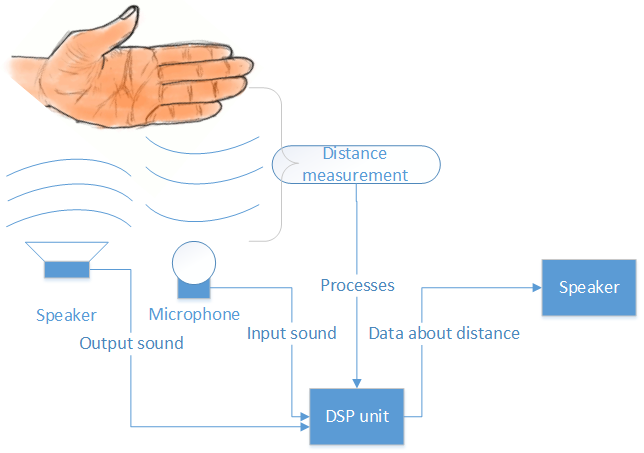
\includegraphics[width=0.6\textwidth]{billeder/systemoverview}
\caption{System sketch}
\label{fig:systemoverview}
\end{figure}

\subsection{System description:}
The system should measure distance using audio. There needs to be a transmitter and a receiver.\\
It should output the distance as a function of either frequency output or LED indication.\\
The system needs to be real-time and measurement and output should be continuous.\\
The user uses his/her hand to place it over the transmitter and receiver to indicate some kind of distance.\\
\subsection{System demands:}
\begin{itemize}
\item Use of DSP
\item Sound output
\item Sound input
\item Precision <5cm
\item Range 10cm-100cm
\item Frequency band: 10kHz-15kHz
\item Sample rate: 48kHz
\item Memory: 1MB
\item System must be real-time
\end{itemize}